\textbf{Pour cette première partie, aucune justification n'est demandée et une seule réponse est possible par question. Pour chaque question, reportez son numéro sur votre copie et indiquez votre réponse.}

	Une réponse fausse ou l'absence de réponse n'enlève aucun point.

\bigskip

Pour cette première partie, aucune justification n'est demandée et une seule réponse est possible par question. Pour chaque question, reportez son numéro sur votre copie et indiquez votre réponse.

Une réponse fausse ou l'absence de réponse n'enlève aucun point.

\medskip
\textbf{\underline{Question 1}}

\medskip
Soient $A$ et $B$ deux événements.


On donne l'arbre de probabilités ci-contre :

\begin{center}
	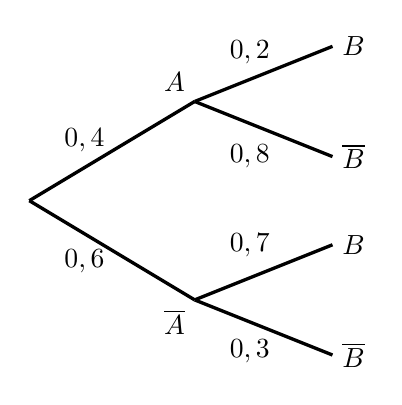
\begin{tikzpicture}[scale=0.7,>=stealth]
		
		
		\coordinate (O) at (0,0);
		
		
		\coordinate (A) at (3,1.8);
		\coordinate (Abar) at (3,-1.8);
		
		
		\coordinate (B1) at (5.5,2.8);
		\coordinate (Bbar1) at (5.5,0.8);
		
		
		\coordinate (B2) at (5.5,-0.8);
		\coordinate (Bbar2) at (5.5,-2.8);
		
		
		\draw[line width=1.2pt] (O) -- (A);
		\draw[line width=1.2pt] (O) -- (Abar);
		
		\draw[line width=1.2pt] (A) -- (B1);
		\draw[line width=1.2pt] (A) -- (Bbar1);
		
		\draw[line width=1.2pt] (Abar) -- (B2);
		\draw[line width=1.2pt] (Abar) -- (Bbar2);
		
		
		\node at (1.0,1.1) {$0,4$};
		\node at (1.0,-1.1) {$0,6$};
		
		
		\node at (4.0,2.7) {$0,2$};
		\node at (4.0,0.8) {$0,8$};
		\node at (4.0,-0.80) {$0,7$};
		\node[below]at (4.0,-2.35) {$0,3$};
		
		
		\node[above left] at (A) {$A$};
		\node[below left] at (Abar) {$\overline{A}$};
		
		\node[right] at (B1) {$B$};
		\node[right] at (Bbar1) {$\overline{B}$};
		\node[right] at (B2) {$B$};
		\node[right] at (Bbar2) {$\overline{B}$};
		
	\end{tikzpicture}
\end{center}
On peut alors affirmer que $P(\overline{A}\cap B)$ est égale à :

\begin{center}
\begin{tblr}{colspec={X[c]X[c]X[c]X[c]},hlines,vlines,width=\linewidth}
\textbf{a.} 1,3 & \textbf{b.} 0,42 & \textbf{c.} 0,7 & \textbf{d.} 0,18 \\
\end{tblr}
\end{center}

\medskip
\textbf{\underline{Question 2}}

\medskip
Dans un lycée, 150 élèves de première générale suivent la spécialité Mathématiques

ce qui représente $\dfrac{3}{5}$ de l'ensemble des élèves de première générale.

\medskip
Le nombre d'élèves en première générale dans ce lycée est :

\begin{center}
\begin{tblr}{colspec={X[c]X[c]X[c]X[c]},hlines,vlines,width=\linewidth}
\textbf{a.} 90 & \textbf{b.} 200 & \textbf{c.} 250 & \textbf{d.} 300 \\
\end{tblr}
\end{center}

\medskip
\textbf{\underline{Question 3}}

\medskip
On considère les nombres $A=\dfrac{1}{3}$ et $B=\dfrac{5}{6}$.

Le nombre $\dfrac{A}{B}+1$ est égal à :

\begin{center}
\begin{tblr}{colspec={X[c]X[c]X[c]X[c]},hlines,vlines,width=\linewidth}
\textbf{a.} $\dfrac{7}{5}$ & \textbf{b.} $\dfrac{3}{5}$ & \textbf{c.} $\dfrac{23}{18}$ & \textbf{d.} $\dfrac{7}{3}$ \\
\end{tblr}
\end{center}

\textbf{\underline{Question 4}}

\medskip
Dans un repère orthonormé $(O\ ;\ \vec{\imath}\ ,\ \vec{\jmath})$, la droite $d$ d'équation réduite $y=\dfrac{1}{3}x+1$ est représentée par :

\begin{center}
	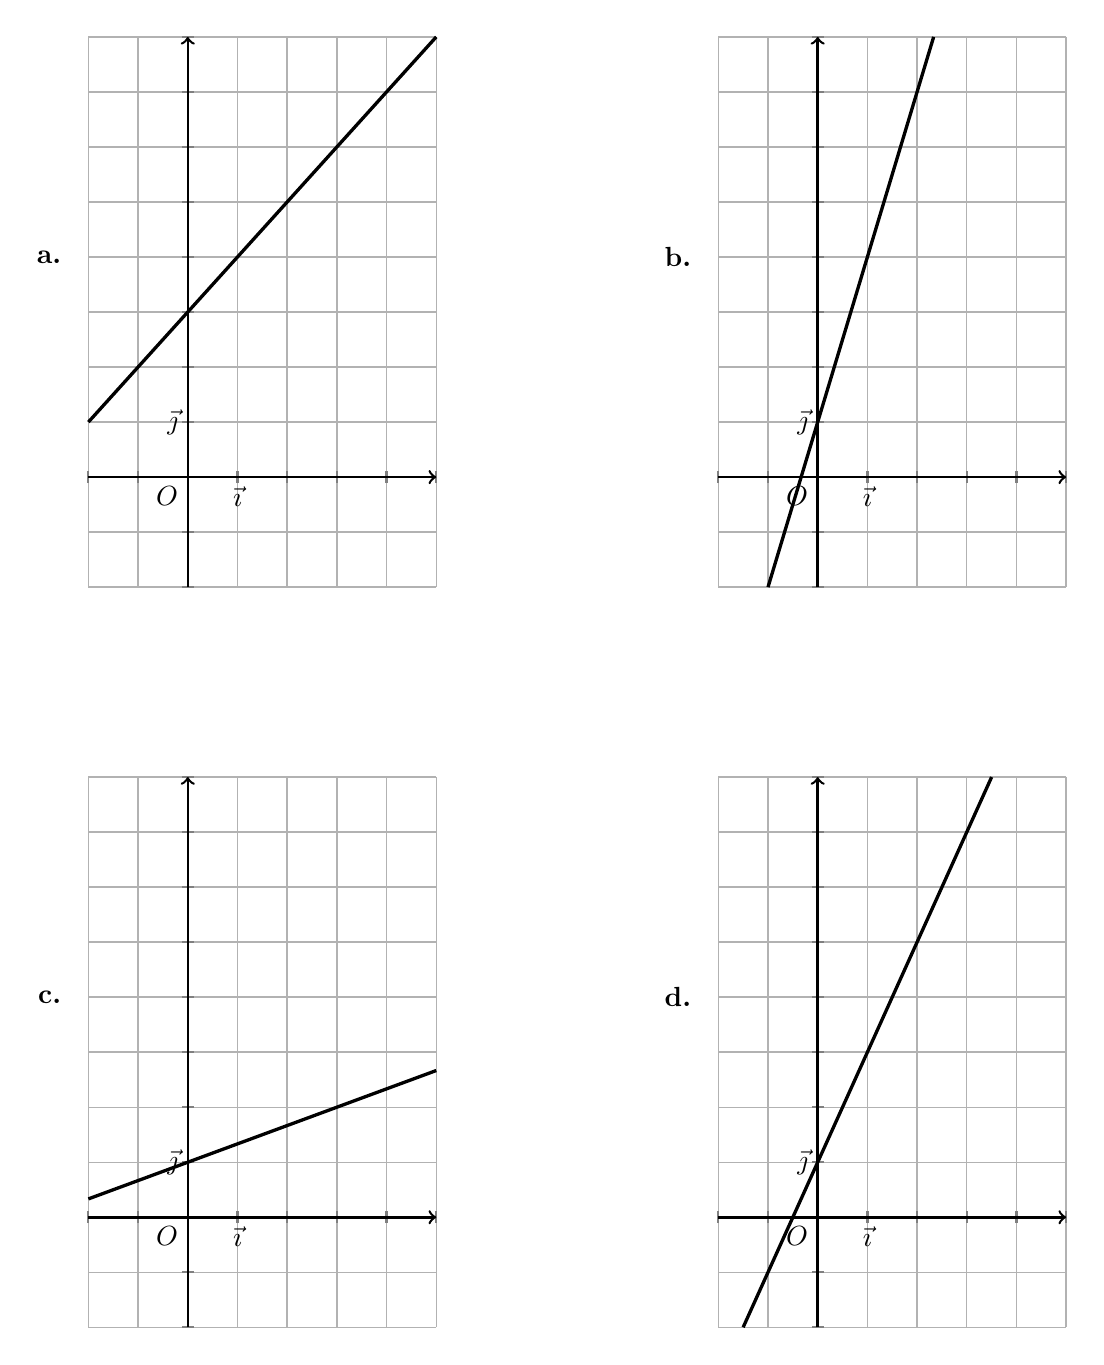
\begin{tikzpicture}
		
		\pgfplotsset{
			monrepere/.style={
				width=6cm,
				height=8.57cm,
				xmin=-2, xmax=5,
				ymin=-2, ymax=8,
				axis lines=middle,
				axis line style={->, line width=0.9pt},
				xtick={-2,-1,0,1,2,3,4,5},
				ytick={-2,-1,0,1,2,3,4,5,6,7,8},
				xticklabels=\empty,
				yticklabels=\empty,
				tick style={line width=0.8pt},
				grid=major,
				grid style={line width=0.5pt, gray!60},
				minor tick num=0,
				clip=false
			}
		}
		
		
		
		
		\begin{axis}[
			monrepere,
			at={(0cm,9.4cm)},
			anchor=south west
			]
			\addplot[domain=-2:5, samples=2, very thick] {x+3};
			\node[font=\bfseries, anchor=east] at (axis cs:-2.35,4) {a.};
			\node[below left] at (axis cs:0,0) {$O$};
			\node[below] at (axis cs:1,0) {$\vec{\imath}$};
			\node[left] at (axis cs:0,1) {$\vec{\jmath}$};
		\end{axis}
		
		
		
		
		\begin{axis}[
			monrepere,
			at={(8cm,9.4cm)},
			anchor=south west
			]
			\addplot[domain=-1:7/3, samples=2, very thick] {3*x+1};
			\node[font=\bfseries, anchor=east] at (axis cs:-2.35,4) {b.};
			\node[below left] at (axis cs:0,0) {$O$};
			\node[below] at (axis cs:1,0) {$\vec{\imath}$};
			\node[left] at (axis cs:0,1) {$\vec{\jmath}$};
		\end{axis}
		
		
		
		
		\begin{axis}[
			monrepere,
			at={(0cm,0cm)},
			anchor=south west
			]
			\addplot[domain=-2:5, samples=2, very thick] {x/3+1};
			\node[font=\bfseries, anchor=east] at (axis cs:-2.35,4) {c.};
			\node[below left] at (axis cs:0,0) {$O$};
			\node[below] at (axis cs:1,0) {$\vec{\imath}$};
			\node[left] at (axis cs:0,1) {$\vec{\jmath}$};
		\end{axis}
		
		
		
		
		\begin{axis}[
			monrepere,
			at={(8cm,0cm)},
			anchor=south west
			]
			\addplot[domain=-1.5:3.5, samples=2, very thick] {2*x+1};
			\node[font=\bfseries, anchor=east] at (axis cs:-2.35,4) {d.};
			\node[below left] at (axis cs:0,0) {$O$};
			\node[below] at (axis cs:1,0) {$\vec{\imath}$};
			\node[left] at (axis cs:0,1) {$\vec{\jmath}$};
		\end{axis}
		
	\end{tikzpicture}
\end{center}
\medskip
\textbf{\underline{Question 5}}

\medskip
La forme développée de $(x^3-1)^2$ est :

\begin{center}
\begin{tblr}{colspec={X[c]X[c]},hlines,vlines,width=\linewidth}
\textbf{a.}\quad $x^6-1$ & \textbf{b.}\quad $x^6-2x^3+1$ \\
\textbf{c.}\quad $x^5-2x^3+1$ & \textbf{d.}\quad $x^6+2x^3-1$ \\
\end{tblr}
\end{center}

\medskip
\textbf{\underline{Question 6}}

\medskip
L'évolution globale correspondant à une hausse de 20 \% puis une baisse de 50 \%, est une baisse de :

\begin{center}
\begin{tblr}{colspec={X[c]X[c]X[c]X[c]},hlines,vlines,width=\linewidth}
\textbf{a.} 10 \% & \textbf{b.} 30 \% & \textbf{c.} 40 \% & \textbf{d.} 60 \% \\
\end{tblr}
\end{center}

\clearpage
\textbf{\underline{Question 7}}

\medskip
Ce tableau donne les résultats partiels d'un sondage dans une classe de première comptant 25 élèves :

\begin{center}
\begin{tblr}{colspec={Q[c,m]Q[c,m]Q[c,m]},hlines,vlines,width=0.7\linewidth,
cell{1}{1}={white},cell{1}{2-3}={gray!45},cell{2-3}{1}={gray!45}}
 & \textbf{16 ans ou moins} & \textbf{Plus de 16 ans} \\
\textbf{\shortstack{Suivent la spécialité\\ Mathématiques}} & 8 &  \\
\textbf{\shortstack{Ne suivent pas la spécialité\\ Mathématiques}} & 7 & 4 \\
\end{tblr}
\end{center}

On interroge un élève de cette classe au hasard.

La probabilité que ce soit un élève qui suive la spécialité Mathématiques sachant qu'il est âgé de plus de 16 ans est :

\begin{center}
\begin{tblr}{colspec={X[c]X[c]X[c]X[c]},hlines,vlines,width=\linewidth}
\textbf{a.} $\dfrac{3}{7}$ & \textbf{b.} $\dfrac{6}{25}$ & \textbf{c.} 6 & \textbf{d.} $\dfrac{3}{5}$ \\
\end{tblr}
\end{center}

\medskip
\textbf{\underline{Question 8}}

\medskip
Soient $x$ et $y$ deux réels strictement positifs tels que : \quad $x=\dfrac{5}{2+y}$

On peut affirmer que :

\begin{center}
\begin{tblr}{colspec={X[c]X[c]X[c]X[c]},hlines,vlines,width=\linewidth}
\textbf{a.} $y=\dfrac{10}{2x-5}$ & \textbf{b.} $y=\dfrac{5}{2+x}$ & \textbf{c.} $y=5-2x$ & \textbf{d.} $y=\dfrac{5}{x}-2$ \\
\end{tblr}
\end{center}

\clearpage
